\section{两类曲线积分的对比和意义}

本节首先对比两类曲线积分,分析它们的区别,再讨论它们的物理意义。

本节要点:
\begin{itemize}
    \item 理解“对弧长”和“对坐标轴”的含义;
    \item 理解曲线积分的物理意义。
\end{itemize}

%============================================================
\subsection{曲线积分的对比}

将三重积分和两类曲线积分放在一起,
\begin{align*}
&\iiint\limits_V{f\left( \boldsymbol{p} \right) dv} \\
&\int\limits_L{f\left( \boldsymbol{p} \right) dl}=\int\limits_L{f\cdot \sqrt{\left( x' \right) ^2+\left( y' \right) ^2+\left( z' \right) ^2}\cdot dt} \\
&\int\limits_L{\left[ \boldsymbol{f}\left( \boldsymbol{p} \right) ^T\mathbf{n}\left( \boldsymbol{p} \right) \right] \cdot dl}=\int\limits_L{\boldsymbol{f}\left( \boldsymbol{p} \right) ^T\boldsymbol{dl}}=\int\limits_L{Pdx+Qdy+Rdz}
\end{align*}
可以看到:
\begin{itemize}
    \item 第一类曲线积分和三重积分的区别只在积分区域,前者是曲线,后者是三维体;
    \item 第一类曲线积分的积分区域是一条曲线,所以又称{\bf 对弧长的曲线积分};
    \item 由于第二类曲线积分又可以写成坐标轴分量的形式,所以又称{\bf 对坐标轴的曲线积分};
    \item 第二类曲线积分和第一类曲线积分的区别在于被积函数,第二类曲线积分的被积函数是向量值函数在曲线切向方向上的投影;
    \item 计算方法上,都是化成一元积分求解。
\end{itemize}

\begin{figure}[h]
\centering
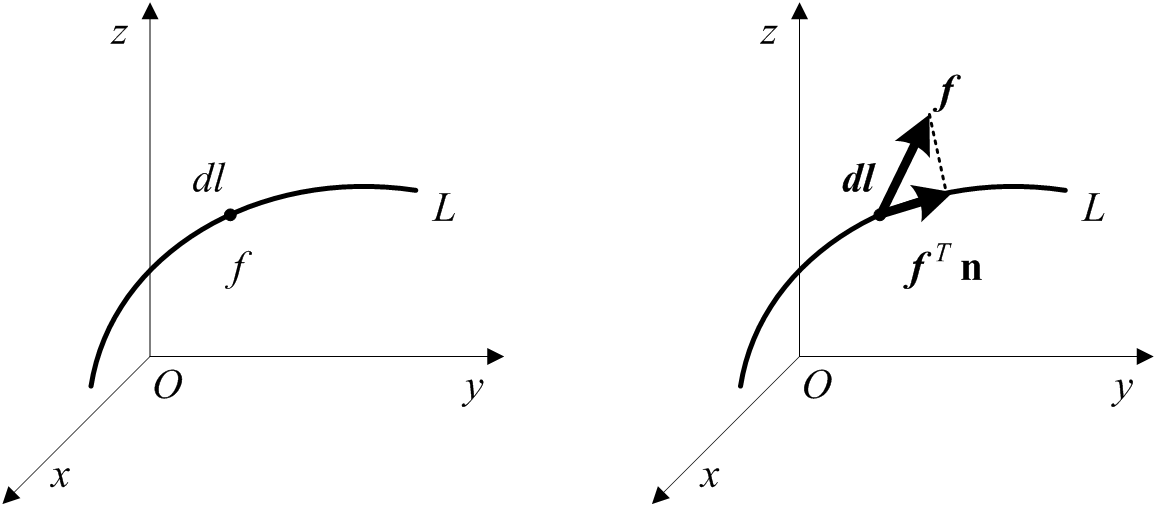
\includegraphics[height=3.5cm]{9.1.png}
\end{figure}

\begin{tcolorbox}
从式子上看,只要看到$dl$的,都是第一类曲线积分,有$dx,dy,dz$单独出现的,就是第二类曲线积分。
\end{tcolorbox}

%============================================================
\subsection{曲线积分的物理意义}

物理上,第一类曲线积分表示一个数量场对一段弧的积分,如绳的质量、非均匀带电曲线的电荷总量等。
第二类曲线积分是对一个矢量场进行环流积分,即求矢量场$\boldsymbol{f}\left( \boldsymbol{p} \right) $在沿某一环流$L$下的环流量。
如果矢量场是力场,则环流积分就是力沿该曲线作的功,如果矢量场是电场,则环流积分就是电势差。

%============================================================
\subsection{计算方法对比}

假设曲线
\[
L:\begin{cases}
	x=x\left( t \right)\\
	y=y\left( t \right)\\
	z=z\left( t \right)\\
\end{cases} \quad t\in \left[ t_1,t_2 \right]
\]
第一类曲线积分和第二类曲线积分:
\begin{align*}
&\begin{cases}
	\int_L{f\left( \boldsymbol{p} \right) dl}\\
	dl=\sqrt{\left( x' \right) ^2+\left( y' \right) ^2+\left( z' \right) ^2}\cdot dt\\
\end{cases} \\
&\Rightarrow \int\limits_L{f\left( \boldsymbol{p} \right) dl}=\int_{t_1}^{t_2}{\left[ f\left( t \right) \cdot \sqrt{\left( x' \right) ^2+\left( y' \right) ^2+\left( z' \right) ^2} \right] dt} \\
&\begin{cases}
	\int_L{\boldsymbol{f}\left( \boldsymbol{p} \right) ^T\boldsymbol{dl}}\\
	\boldsymbol{dl}=\mathbf{n}dl=\left( x'\,\,y'\,\,z' \right) ^Tdt\\
\end{cases} \\
&\Rightarrow \int\limits_L{\boldsymbol{f}\left( \boldsymbol{p} \right) ^T\boldsymbol{dl}}=\int_{t_1}^{t_2}{\left[ P\left( t \right) \cdot x'+Q\left( t \right) \cdot y'+R\left( t \right) \cdot z' \right] dt}
\end{align*}



